\chapter{Introduction}
\label{chapter:introduction}

One of the main goals in computer graphics is realistic rendering. 
Even though computer graphics is constantly improving, we are still quite away from reality because material representation in a traditional way lack important realistic properties. 
A 2-D texture in conjunction with a shading model is a conventional way to represent material appearance in rendering.
On the other side, real-world materials surfaces consist of surface meso-structures, i.e. intermediate in size local geometric details.
Meso-structures are responsible for fine-scale shadows, self-occlusions, inter-reflection, subsurface scattering and specularities.
Also, reflectance of the real-world materials spatially varies.

One of the possible solution to represent such material's attributes is to use sophisticated light functions, for instance a Bidirectional Texture Function (BTF). 
A BTF is a 6-dimensional function that depends on camera and light directions as well as on spatial texture coordinates. 
BTFs conceptually extend traditional 2-D texture by the dependence on light and camera directions.
This function is usually acquired as a data-set of thousands images that cover varying light and camera directions.
Due to enormous size of such data direct rendering on the modern hardware without any compression is impractical.
Fortunately, compression methods combined with modern graphics hardware provide fast computational speed, which allows us to employ BTF.



\section{Outline}
\label{section:outline}

\begin{figure}[h]
 \centering
 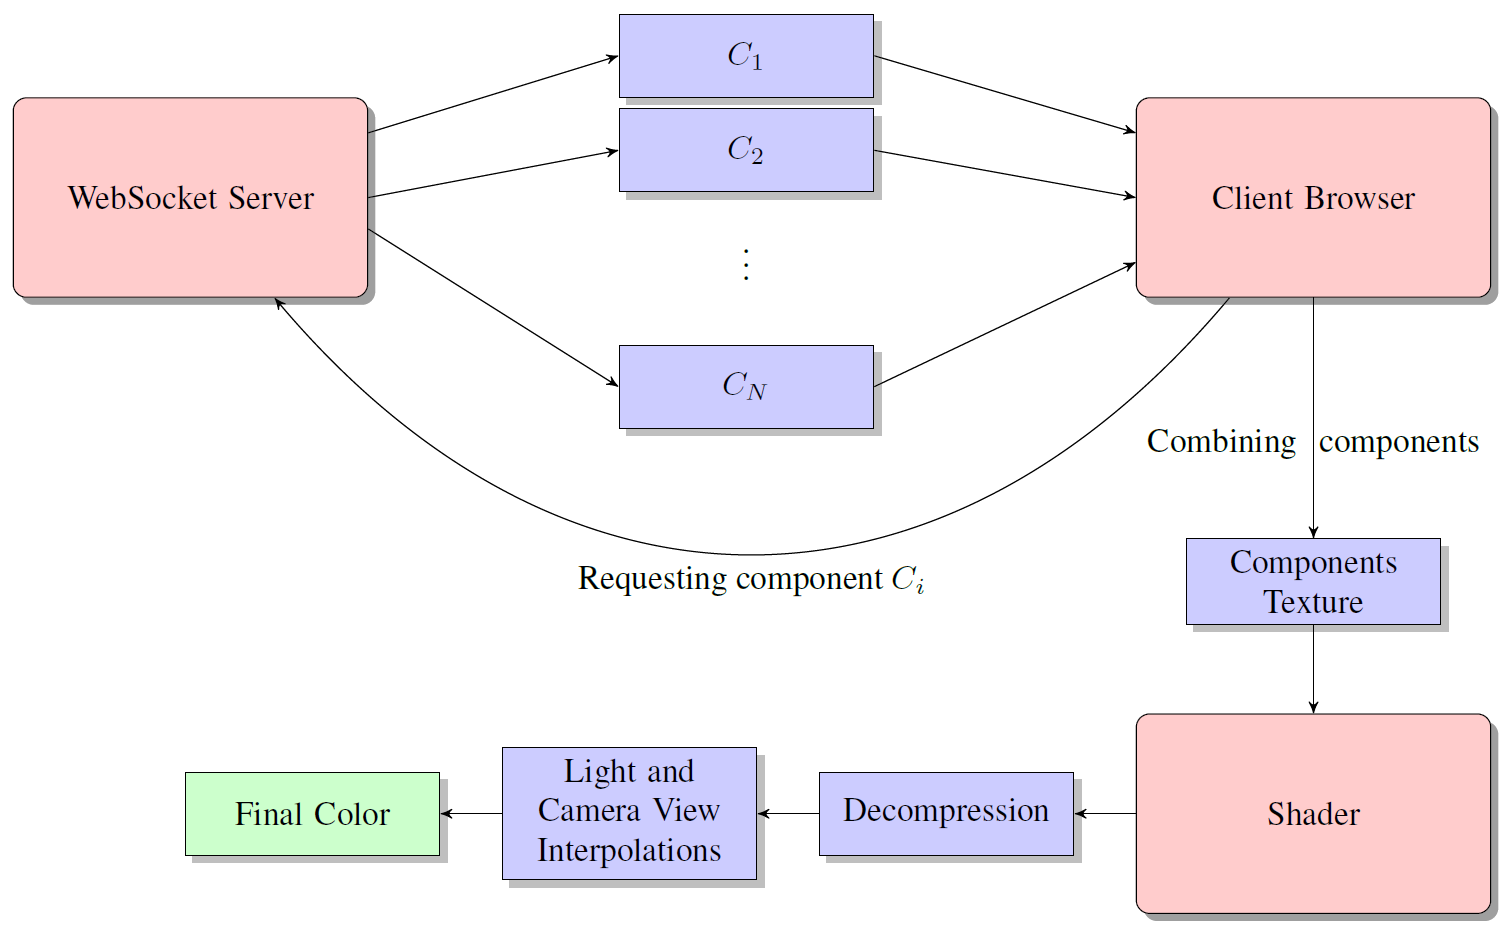
\includegraphics[width=1.0\textwidth]{figures/overview}
 \caption[Model Overview ] {
 	{\bf Model Overview}

	
	}
 \label{fig:overview}
\end{figure}



